
\section{CROW}
\label{section:crow}

This section describes CROW \cite{CROW}, our first contribution. CROW is a tool tailored to create semantically equivalent \wasm variants out of a single program, either C/C++ and Rust code or LLVM bitcode.
In \autoref{diagrams:crow}, we describe the workflow of CROW to create program variants.
The figure highlights the main two stages of the CROW's workflow, \textit{exploration} and \textit{combining}. The workflow starts by compiling the input program into the LLVM bitcode using clang from the source code. During the \emph{exploration} stage, CROW takes an LLVM bitcode and, for its code blocks, produces a collection of code replacements that are functionally equivalent to the original program. 
%In the following, we enunciate the definitions we use along with this work for a code block, functional equivalence, and code replacement. 
In the \emph{combining} stage, CROW combines the code replacements to generate different LLVM bitcode variants. 
Then, a variant bitcode is compiled into a \wasm binary if requested. Finally, CROW generates the variants from all possible combinations of code replacements as the power set of all code replacements.  

%\subsection*{Overview}

\begin{figure*}[h]
    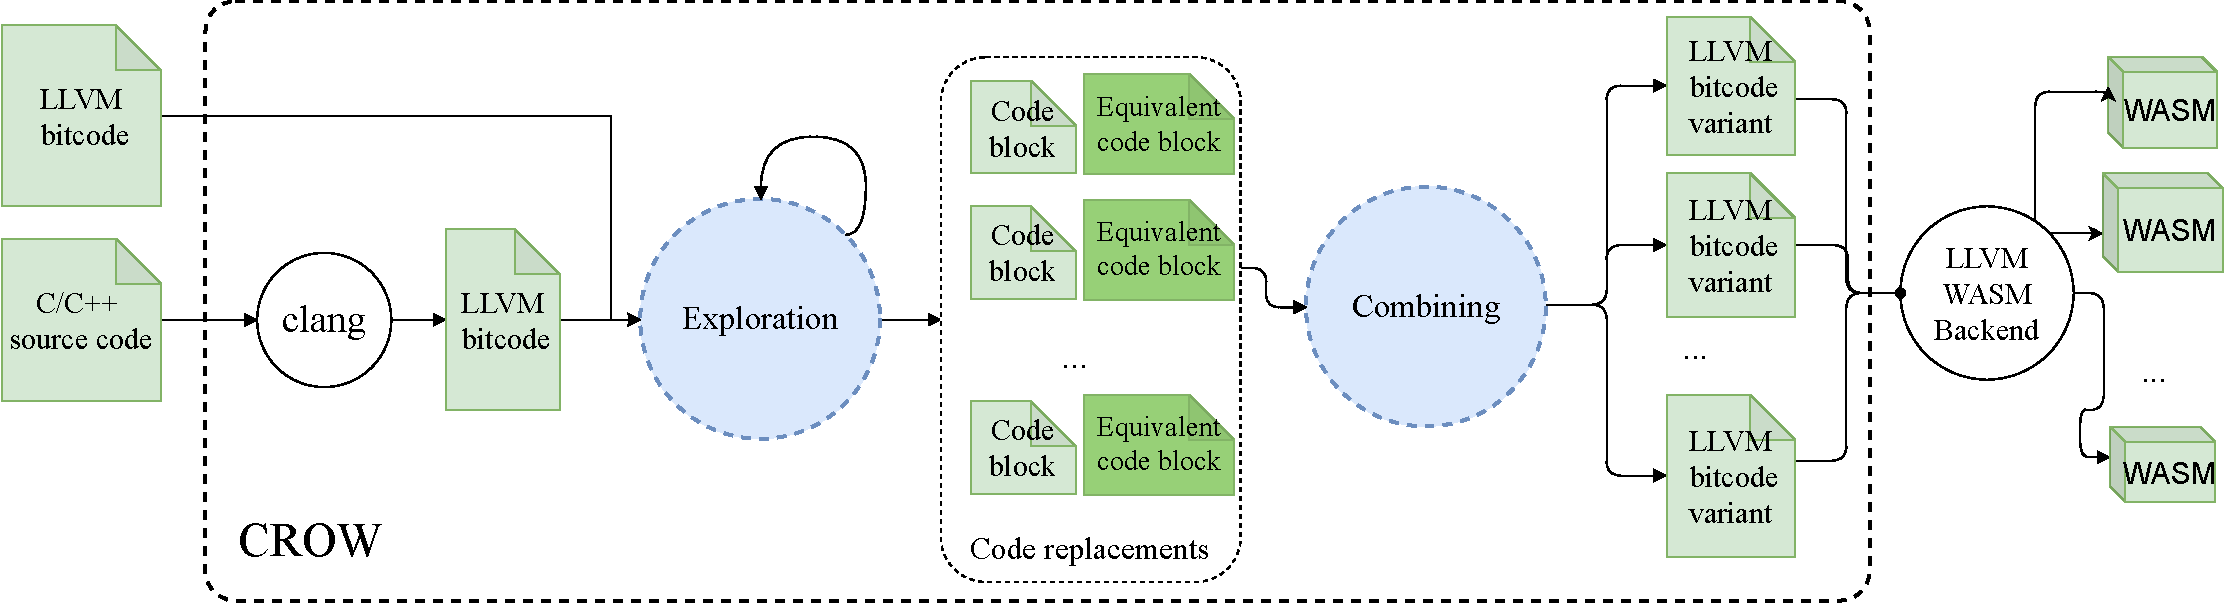
\includegraphics[width=\linewidth]{diagrams/generation/crow.drawio.pdf}
    \caption{CROW workflow to generate program variants. CROW takes C/C++ source codes or LLVM bitcodes to look for code blocks that can be replaced by semantically equivalent code and generates program variants by combining them.}
    \label{diagrams:crow}
\end{figure*}



%CROW operates at the code block level, taking them from the functions defined inside the input LLVM bitcode module. 
%In addition, the retargeted superoptimizer is in charge of finding the potential places in the original code blocks where a replacement can be applied. Finally, we use the enumerative synthesis strategy of the retargeted superoptimizer to generate code replacements.
%The code replacements generated through synthesis are verified, according to \autoref{def:functional-equivalence}, by internally using a theorem prover. 

\begin{comment}

\begin{definition}{Block (based on Aho \etal \cite{ahodragonbook}):}\label{def:code-block}
    Let $P$ be a program. A block $B$ is a grouping of declarations and statements in $P$ inside a function $F$. 
\end{definition}

\todo{Move to chapter 2}

\begin{definition}{Functional equivalence modulo program state (based on Cohen \etal \cite{cohen1993operating}):}
    \label{def:functional-equivalence}
    Let $B_1$ and $B_2$ be two code blocks according to \autoref{def:code-block}. We consider the program state before the execution of the block, $S_i$, as the input and the program state after the execution of the block, $S_o$, as the output. $B_1$ and $B_2$ are functionally equivalent if given the same input $S_i$ both codes produce the same output $S_o$.
\end{definition}

\begin{definition}{Code replacement:}
    \label{def:code-replacement}
    Let $P$ be a program and $T$ a pair of code blocks $(B_1, B_2)$. $T$ is a candidate code replacement if $B_1$ and $B_2$ are both functionally equivalent as defined in \autoref{def:functional-equivalence}.
    Applying $T$ to $P$ means replacing $B_1$ by $B_2$. The application of $T$ to $P$ produces a program variant $P'$ which consequently is functionally equivalent to $P$.     
\end{definition}
\end{comment}

\subsection*{Variants' generation}

CROW is based on the work of Jacob \etal \cite{jacob2008superdiversifier}. Their work uses code superoptimization to generate software diversification with an approach called superdiversification. 
% How a superoptimizer works
Code superoptimization focuses on \emph{searching} for a new program which is faster or smaller than the original code, while preserving its functionality.
The concept of superoptimizing a program dates back to 1987, with the seminal work of Massalin \cite{Massalin1987} which proposes an exhaustive exploration of the solution space. The search space is defined by choosing a subset of the machine's instruction set and generating combinations of optimized programs, sorted by length in ascending order. If any of these programs are found to perform the same function as the source program, the search halts. The main difference between the superoptimization process and a superdiversifier it that the latter keeps intermediate search results for the sake of diversification. 

We use the seminal work of Jacob and colleagues to implement CROW because of two main reasons.
First, the code replacements generated by this technique outperform diversification strategies based on hand-written rules. Besides, this technique is fully automatic.
Second, there is a battle tested superoptimizer for LLVM, Souper \cite{Sasnauskas2017Souper:Superoptimizer}. It dates from 2017 and has an active community of maintainers. By extending Souper with superdiversification, it allows us to contribute with a new mutation strategy, \emph{constant inferring} (in addition to the before mentioned strategies in \autoref{sota:sota}) to artificially generate diversification. We modify it to keep the intermediate solutions in their searching algorithm to generate program variants. Besides, 
we prevent Souper from synthesizing instructions that have no correspondence in the \wasm backend to reduce the searching space for variants. In addition, we disable the majority of the pruning strategies of Souper for the sake of more variants. Our modified version of Souper can be found at \todo{}.

% Souper
%Souper is an state-of-the-art superoptimizer for LLVM. It enumerates a set of several optimization candidates to be replaced.
%Souper is based on a Satisfiability Modulo Theories (SMT) solver. SMT solvers are useful for both verification and synthesis of programs \cite{10.1007/978-3-540-78800-3_24}.

%We implement the \emph{exploration} stage of CROW by retargeting Souper. The main objective of Souper is to find the best (smallest) possible program,  

\subsection*{Constant inferring}

As we previously mentioned, extending Souper as a superdiversifier contributes with a new mutation strategy called \emph{constant inferring}. 
The main component of Souper infers pieces of code as a single constant assignment particularly for boolean valued variables that are used to control branches.
If a program branching is removed due to a constant inferring, the generated program is considerably different to the original program, statically and dynamically.
Let us illustrate the case with an example.
The Babbage problem code is composed of a loop which stops when it discovers the smaller number that fits with the Babbage condition below.
\begin{center}
\begin{tabular}{c}

\lstset{language=C++,
                    style=CStyle,
                    basicstyle=\small\ttfamily,
                    columns=fullflexible,
                    breaklines=true, 
                    postbreak=\mbox{\textcolor{red}{$\hookrightarrow$}\space}}
\begin{lstlisting}[]
while((n * n) % 1000000 != 269696) n++;
\end{lstlisting}
\end{tabular}
\end{center}
% llvm-opt: rool unroll
In theory, this value can also be inferred by unrolling the loop the correct number of times with traditional tools like llvm-opt.
However, llvm-opt cannot unroll a \texttt{\textbf{while}}-loop because the loop count is too large.
% Souper
On the other hand, Souper can deal with this case, inferring the value of $n$ such that the Babbage condition is reached. Therefore, since the condition in the loop will always be false, the loop is dead code, and is removed in the final compilation. It is clear that the new program is remarkably different, smaller and faster than the original code.

When we retarget Souper we recombine all found replacements to create new programs, including those for which a constant inferring was performed.
This allows to create variants that are also better than the original program in terms of size and performance.

\subsection*{Removing latter optimizations for LLVM}

During the implementation of CROW we have the premise of removing all builtin optimizations in the LLVM compiler that could reverse Wasm variants.
Therefore, in addition to the extension of Souper, we modify the LLVM compiler and the \wasm backend.
We disable all optimizations in the \wasm backend that could reverse the superoptimizer transformations, such as constant folding and instructions normalization.


%\todo{We disable cost restrictions and the LLVM backend optimizations...maybe for the assesment RQ ?}

\subsection*{CROW instantiation}
%\label{section:crow:example}
%In \autoref{section:crow} we describe the main components and contributions of CROW. In this section we instantiate the workflow presented in \autoref{workflow} from the input of an example C code to the generation of a pool of \wasm program variants.

Let us illustrate how CROW works with the simple example code in \autoref{CExample}. The \texttt{f} function calculates the value of $2 * x + x$ where \texttt{x} is the input for the function.  CROW compiles this source code and generates the intermediate LLVM bitcode in the left most part of \autoref{example:crow:original:llvm}. CROW potentially finds two code blocks to look for variants, as the right-most part of \autoref{example:crow:original:llvm} shows.

% snippet of code showing the detection of code blocks
    
\begin{code}
    \lstset{language=C,
    basicstyle=\small\ttfamily,caption={C function that calculates the quantity $2x + x$},label=CExample}
    \begin{lstlisting}[style=CStyle]
int f(int x) { 
    return 2 * x + x; 
}    
    \end{lstlisting}
    
\end{code}

\lstdefinelanguage{LLVM}
    {morekeywords={i32,mul,align,nsw,add,load,store,define,br, ret, shl, ret},
    sensitive=false,
    morecomment=[l]{;},
    morecomment=[s]{;}{;},
    morestring=[b],
}
\lstdefinestyle{nccode}{
    numbers=left,
    tabsize=4,
    showspaces=false,
    breaklines=true, 
    showstringspaces=false,
    moredelim=**[is][{\btHL[fill=black!10]}]{`}{`},
    moredelim=**[is][{\btHL[fill=celadon!40]}]{!}{!}
}
\lstset{
    language=LLVM,
    style=nccode,
    %basicstyle=\small\ttfamily,
    columns=fullflexible,
    breaklines=true
}


\begin{code}
    \centering
    \captionof{lstlisting}{LLVM's intermediate representation program, its extracted instructions and replacement candidates. Gray highlighted lines represent original code, green for code replacements. }\label{example:crow:original:llvm}
    \lstset{numbers=none}
    \noindent\begin{minipage}[t]{.33\linewidth}
    \centering
    \begin{lstlisting}[xleftmargin=1em,escapechar=?]
    define i32 @f(i32) {

    ?\tikzmarkWS{2}{code 2}{11.5}{10}{3.5cm}?
    ?\tikzmarkWS{1}{code 1}{11.5}{3.5}{3.0cm}?
    %2 = mul nsw i32 %0,2
    %3 = add nsw i32 %0,%2 

    ret i32 %3
    }
    
    define i32 @main() {
    %1 = tail call i32 @f(i32 10)
    ret i32 %1
    }
    \end{lstlisting}
    \end{minipage}%\hfill%
    \begin{minipage}[t]{.32\linewidth}
        \begin{lstlisting}[xleftmargin=1em,escapechar=?]
?Replacement candidates for code\_1?

`%2 = mul nsw i32 %0,2`

!%2 = add nsw i32 %0,%0!

!%2 = shl nsw i32 %0, 1:i32!
    \end{lstlisting}
    \end{minipage}%\hfill%
    \begin{minipage}[t]{.32\linewidth}
        \lstdefinestyle{nccode}{
        tabsize=4, 
        showspaces=false,
        breaklines=true, 
        showstringspaces=false,
        moredelim=**[is][{\btHL[fill=black!10]}]{`}{`},
        moredelim=**[is][{\btHL[fill=celadon!40]}]{!}{!}
        }
        \lstset{
            language=LLVM,
            style=nccode,
            columns=fullflexible,
            breaklines=true,
            belowcaptionskip=1pt,
            abovecaptionskip=1pt,
        } 
        \begin{lstlisting}[name={B},escapechar=?]
?Replacement candidates for code\_2?

`%3 = add nsw i32 %0,%2`

!%3 = mul nsw %0, 3:i32!
        \end{lstlisting}
    \end{minipage}
    
\end{code}





\begin{code}
    \centering
    \captionof{lstlisting}{Candidate code replacements combination. Orange highlighted code illustrate replacement candidate overlapping.}\label{example:crow:original:combination}
    \lstset{numbers=none}
    \noindent\begin{minipage}[t]{.5\linewidth}
    \begin{lstlisting}[xleftmargin=1em,escapechar=?]
`%2 = mul nsw i32 %0,2`
`%3 = add nsw i32 %0,%2`

!%2 = add nsw i32 %0,%0!
`%3 = add nsw i32 %0,%2`

!%2 = shl nsw i32 %0, 1:i32!
`%3 = add nsw i32 %0,%2`

    \end{lstlisting}
    \end{minipage}%\hfill%
    \begin{minipage}[t]{.5\linewidth}
        \lstdefinestyle{nccode}{
        tabsize=4, 
        showspaces=false,
        breaklines=true, 
        showstringspaces=false,
        moredelim=**[is][{\btHL[fill=black!10]}]{`}{`},
        moredelim=**[is][{\btHL[fill=celadon!40]}]{!}{!},
        moredelim=**[is][{\btHL[fill=weborange!40]}]{'}{'}
        }
        \lstset{
            language=LLVM,
            style=nccode,
            columns=fullflexible,
            breaklines=true,
            belowcaptionskip=1pt,
            abovecaptionskip=1pt,
        } 
        \begin{lstlisting}[xleftmargin=1em,escapechar=?]
'%2 = mul nsw i32 %0,2'
!%3 = mul nsw %0, 3:i32!

'%2 = add nsw i32 %0,%0'
!%3 = mul nsw %0, 3:i32!

'%2 = shl nsw i32 %0, 1:i32'
!%3 = mul nsw %0, 3:i32!

    \end{lstlisting}
    \end{minipage}
\end{code}


\begin{tikzpicture}[remember picture,overlay]
%\path (2.north) edge[<-, bend left] (1.north);
%\path[draw, ->] (3.west) edge[<-, bend left] (2.west);
%\path (4.west) edge[<-, bend left] (3.west);
%\path (1.south) edge[<-, bend left] (4.south);

%\path (2.east) edge[<-, bend left, blue] (5.north);
%\path (3.east) edge[<-, bend right, olive] (2.east);
%\path (1.east) edge[<-, bend left, black] (replall1.west);
%\path (2.east) edge[<-, bend left, black] (replall2.west);
%\path (rep11.east) edge[<-, bend left, black] (6.east);
%\path (9.east) edge[<-, bend right, black] (4.east);
%\path (7.east) edge[<-, bend right, black] (8.east);
%\path (5.south) edge[<-, bend right, blue] (4.east);
%\path (9.north) edge[<-] (8.south);
%\path (5.south) edge[<-, bend left] (9.south);


%\path (10.north) edge[<-, bend left] (11.north);
%\path (11.south) edge[<-, bend left] (10.south);
%\path (7) edge[<-, bend right] (6.east);
%\path (8) edge[<-, bend right] (7.east);
\end{tikzpicture}


    

CROW, in the exploration stage detects 2 code blocks, \texttt{code\_block\_1} and \texttt{code\_block\_2} as the enclosing boxes in the left most part of \autoref{example:crow:original:llvm} shows. CROW synthesizes $2 + 1$ candidate code replacements for each code block respectively as the green highlighted lines show in the right most parts of \autoref{example:crow:original:llvm}.
The baseline strategy of CROW is to generate variants out of all possible combinations of the candidate code replacements, \ie uses the power set of all candidate code replacements.

In the example, the power set is the cartesian product of the found candidate code replacements for each code block, including the original ones, as \autoref{example:crow:original:combination} shows. The power set size results in $6$ potential function variants. Yet, the generation stage would eventually generate $4$ variants from the original program. CROW generated 4 statically different Wasm files, as \autoref{example:crow:variants:wasm} illustrates. This gap between the potential and the actual number of variants is a consequence of the redundancy among the bitcode variants when composed into one. In other words, if the replaced code removes other code blocks, all possible combinations having it will be in the end the same program. In the example case, replacing \texttt{code\_block\_2} by \texttt{mul nsw \%0, 3}, turns \texttt{code\_block\_1} into dead code, thus, later replacements generate the same program variants. The rightmost part of \autoref{example:crow:original:combination} illustrates how for three different combinations, CROW produces the same variant. We call this phenomenon a candidate code replacement overlapping.

One might think that a reasonable heuristic could be implemented to avoid such overlapping cases. Instead, we have found it easier and faster to generate the variants with the combination of the replacement and check their uniqueness after the program variant is compiled. This prevents us from having an expensive checking for overlapping inside the CROW code. Still, this phenomenon calls for later optimizations in future works.

\lstdefinestyle{nccode}{
        numbers=none,
        firstnumber=2,
        stepnumber=1,
        numbersep=10pt,
        tabsize=4, 
        showspaces=false,
        breaklines=true, 
        showstringspaces=false,
    moredelim=**[is][\btHL]{`}{`},
    moredelim=**[is][{\btHL[fill=black!10]}]{`}{`},
    moredelim=**[is][{\btHL[fill=celadon!40]}]{!}{!}
}

\lstset{
    language=WAT,
    style=nccode,
    basicstyle=\footnotesize\ttfamily,
    columns=fullflexible,
    breaklines=true
}


\begin{code}
    \centering
    \captionof{lstlisting}{\termidx{Wasm }program variants generated from program \autoref{CExample}.}\label{example:crow:variants:wasm}
    \lstset{numbers=none}
    \noindent\begin{minipage}[t]{.45\linewidth}
    \begin{lstlisting}[xleftmargin=1em,escapechar=?]
func $f (param i32) (result i32)
   local.get 0
    `i32.const 2`
    `i32.mul`
    `local.get 0`
    `i32.add`

        \end{lstlisting}
\begin{lstlisting}[xleftmargin=1em,escapechar=?]
func $f (param i32) (result i32)
    local.get 0
    !local.get 0!
    !i32.add!
    `local.get 0`
    `i32.add`

                \end{lstlisting}
    \end{minipage}\hfill
    \noindent\begin{minipage}[t]{.45\linewidth}
\begin{lstlisting}[xleftmargin=1em,escapechar=?]
func $f (param i32) (result i32)
    local.get 0
    !i32.const 1!
    !i32.shl!
    `local.get 0`
    `i32.add`

    \end{lstlisting}
\begin{lstlisting}[xleftmargin=1em,escapechar=?]
func $f (param i32) (result i32)
    local.get 0
    !i32.const 3!
    !i32.mul!

            \end{lstlisting}
        \end{minipage}
\end{code}



